\documentclass{article}

\usepackage{listings}
\usepackage[dvipsnames]{xcolor}
\usepackage[utf8]{inputenc}
\usepackage{graphicx}
\usepackage{hyperref}
\usepackage{url}
\usepackage{wrapfig}
\usepackage{subfigure}

\title{Profielwerkstuk Documentatie}

\author{Jochem Raat, Marien Raat, Pieter Staal}
\date{September 18, 2015}

\bibliographystyle{plain}

\hypersetup{pdfborder={0 0 0},colorlinks=false}

\lstset{
language=C++,
aboveskip=3mm,
belowskip=3mm,
showstringspaces=false,
columns=flexible,
frame=tb,
basicstyle={\small\ttfamily},
numbers=none,
numberstyle=\tiny\color{Gray},
keywordstyle=\color{Blue},
commentstyle=\color{OliveGreen},
stringstyle=\color{Maroon},
breaklines=true,
breakatwhitespace=true,
tabsize=4
}

\begin{document}
\maketitle
\newpage

\tableofcontents
\newpage

\section{C++ Introductie}

\subsection{Introductie}
Het doel van ons profielwerkstuk is om een programma te schrijven dat eilanden genereert. Dit doen we (grotendeels) in de taal C++. Om de code te lezen is het dus handig om wat basiskennis van C++ te hebben en die zullen we in dit hoofdstuk proberen te geven. De versie van C++ die we gebruiken is C++11. C++11 is een versie van C++ die in 2011 is goedgekeurd door de ISO (de Internationale Organisatie voor Standaardisatie). We hebben deze versie gekozen omdat deze oud genoeg is om goed ondersteund te worden, maar ook nieuw genoeg om vele goede functies te hebben. De belangrijkste functie die we nodig hadden uit C++11 was een goede pseudo-willekeurigheid generator, over deze generator vertellen we verderop meer.

\subsection{Objectgeoriënteerd programmeren}
Om C++ code te kunnen lezen moet je eerst meer weten over het objectgeoriënteerd programmeren, vaak afgekort als OOP van het Engelse Object-Oriented Programming. C++ is namelijk oorspronkelijk ontworpen om aan de programmeertaal C de mogelijkheid voor objectgeoriënteerd programmeren toe te voegen.  De belangrijkste twee concepten in objectgeoriënteerd programmeren zijn klassen en objecten. Een klasse dient als een blauwdruk voor objecten. In een klasse twee soorten informatie over de objecten die eruit kunnen ontstaan worden gedefinieerd:

\begin{itemize}
\item Welke \textit{attributen} het object heeft waarmee de toestand en de eigenschappen van het object worden opgeslagen.
\item Welke \textit{methoden} het object heeft. Deze methoden zijn functies die de attributen van het object kunnen aanpassen of inlezen en daarmee dingen kunnen doen, zoals een van de attributen afdrukken op het scherm.
\end{itemize}

\subsection{Voorbeeld van klassen en objecten}
We zullen de concepten van klassen en objecten proberen te verduidelijken met hulp van een klein voorbeeld. We hebben een klasse \texttt{Persoon} die de attributen naam en \texttt{leeftijd} definieert en de methode \texttt{zegHalloTegen} dat een argument aanneemt, namelijk de \texttt{aangesprokene} waartegen het object hallo moet zeggen. Deze methode zou dan zo kunnen zijn gemaakt dat hij afdrukt: “Hallo \texttt{aangesprokene}, ik ben naam en ik ben \texttt{leeftijd} jaar oud”.


Vervolgens zou je met deze klasse een object \texttt{jan} kunnen initialiseren met de \texttt{naam} “Jan” en de \texttt{leeftijd} 17. Als je tegen dit object dan \texttt{zegHalloTegen} “Bas” zou aanroepen, zou het object het volgende afdrukken: “Hallo Bas, ik ben Jan en ik ben 17 jaar oud”.

\subsection{Objectgeoriënteerd programmeren in C++}
In C++ worden de definities van klassen vaak opgesplitst in een header bestand dat aangeeft welke attributen en methoden de klasse heeft en een apart bestand dat de implementaties van de methoden aangeeft. Ook heeft elke klasse in C++ minimaal één constructor, een speciale functie die een objectkan initialiseren vanuit de klasse. De constructor zou in onze voorbeeld met een klasse voora personen bijvoorbeeld twee argumenten kunnen aannemen, de \texttt{naam} en de \texttt{leeftijd}.

Het header bestand voor de \texttt{Persoon} klasse zou bijvoorbeeld een bestand genaamd “\texttt{persoon.h}” kunnen zijn, omdat het gebruikelijk is om header bestanden de extensie “\texttt{.h}” te geven. De inhoud hiervan zou er als volgt uit kunnen zien

\begin{lstlisting}
// Voorbeeld 1: persoon.h

#include <string>

class Persoon {
public:
  Persoon(std::string naam, int leeftijd);
  void zegHalloTegen(std::string aangesprokene);
private:
  std::string naam;
  int leeftijd;
};
\end{lstlisting}

In dit bestand wordt dus vastgesteld welke attributen en methodes de klasse \texttt{Persoon} bevat. Om te begrijpen hoe dit wordt genoteerd zullen we regel voor regel de code doorlopen.

\begin{lstlisting}[frame=none]
#include <string>
\end{lstlisting}

Regels die beginnen met een hekje ('\texttt{\#}') zijn instructies voor de compiler. De compiler is een programma die de C++ code die we schrijven omzet naar een programma dat kan worden uitgevoerd. In dit geval verteld \texttt{\#include <string>} aan de compiler dat we de module \texttt{string} nodig hebben. Deze gebruiken we verderop namelijk voor het type \texttt{std::string}.

\begin{lstlisting}[frame=none]
class Persoon 
\end{lstlisting}

Dit geeft aan dat we een klasse gaan definiëren met de naam persoon, de definitie van de klasse is alles binnen de accolades ('\texttt{\{}' en '\texttt{\}}').

\begin{lstlisting}[frame=none]
public:
\end{lstlisting}

Dit geeft aan dat de komende regels allemaal over attributen en methodes van de klasse gaan die publiek zijn. Publiek geeft aan dat een methode of attribuut ook door gebruikers van de objecten die vanuit de klasse worden gemaakt kan worden gebruikt. De private attributen en methoden kunnen alleen door methoden van het object zelf worden gebruikt.

\begin{lstlisting}[frame=none]
Persoon(std::string naam, int leeftijd);
\end{lstlisting}

Hier wordt de constructor gedefinieerd, waarmee dus een object van deze klasse kan worden geïnitialiseerd. Je kan zien dat dit de constructor is doordat de naam precies hetzelfde is als de naam van de gehele klasse, namelijk \texttt{Persoon}. Na \texttt{Persoon} staan de twee argumenten die je aan de constructor moet meegeven tussen haakje, gescheiden door een komma.

Het eerste is \texttt{std::string} naam dit geeft een argument aan van het type \texttt{std::string}. Ditis het type waarmee stukjes tekst worden aangegeven in C++, die vaak gewoon kortaf strings worden genoemd. \texttt{std::} geeft aan dat het om het type \texttt{string} gaat dat in de standaard is gedefinieerd (std is kort voor standard), het is vooral belangrijk om te onthouden dat \texttt{std::string} een stukje tekst aangeeft. Achter het type staat de naam van het argument, wat in principe niet belangrijk is voor de klasse, maar wel handig voor de mensen die het lezen om te zien wat het argument aangeeft.

Het tweede is int \texttt{leeftijd}, een argument van het type \texttt{int}. Een int is een integer, dus een geheel getal. Achter \texttt{int} staat wederom de naam van het argument, die ook hier niet belangrijk is, maar wel aangeeft waar het argument voor zal worden gebruikt. Na de argumenten komt de punt- komma om aan te geven dat dit het einde van de definitie van de constructor is.

\begin{lstlisting}[frame=none]
void zegHalloTegen(std::string aangesprokene);
\end{lstlisting}

Hier wordt de eerste (en meteen ook de laatste) echte methode gedefinieerd, namelijk de methode genaamd \texttt{zegHalloTegen}. Voor de naam van de methode staat \texttt{void} dit betekent dat \texttt{zegHalloTegen} niks terug geeft (void betekent leegte in het Engels). Dit heet het return type, dat dus aangeeft wat de methode “\emph{returnt}”. Dit return type is nodig omdat sommige methoden iets terug moeten geven, zodat een andere methode dat kan gebruiken.

Tussen haakjes staan achter de naam de argumenten die deze methode mee moet krijgen gegeven, dit is er in dit geval maar één namelijk \texttt{std::string aangesprokene}. Dit is dus de naam van degene die door het object moet worden begroet. Deze naam is ook weer van het type \texttt{std::string} en geeft dus een stukje tekst aan. Na dit argument volgt de punt-komma om aan te geven dat de definitie van deze methode hier eindigt.

\begin{lstlisting}[frame=none]
private:
\end{lstlisting}

Dit geeft aan dat de volgende definities private attributen en methoden aangeven.

\begin{lstlisting}[frame=none]
std::string naam; 
\end{lstlisting}

Dit is het eerste attribuut van de klasse, genaamd naam. Dit attribuut is van het type \texttt{std::string}, dus weer een stukje tekst. Bij een attribuut is de naam die eraan wordt gegeven in het header bestand wel belangrijk in tegenstelling tot de namen van argumenten van methodes. De naam van een attribuut wordt namelijk gebruikt om dat attribuut te kunnen veranderen of bekijken in de code.

\begin{lstlisting}[frame=none]
int leeftijd;
\end{lstlisting}

Dit is het tweede attribuut van de klasse, met de naam \texttt{leeftijd}. Dit attribuut is van het type \texttt{int}, dus het gaat om een getal.

\begin{lstlisting}[frame=none]
};
\end{lstlisting}

Een sluitende accolade gevolgd door een punt-komma geeft het eind van de definitie van attributen en methoden van de klasse aan. Nu gaan we kijken naar het bestand dat de methoden en de \texttt{constructor} ook echt definieert. Dit bestand zou bijvoorbeeld “\texttt{persoon.cpp}” kunnen heten. De extensie “\texttt{.cpp}” (“\texttt{.cpp}” staat voor \emph{C Plus Plus}) is gebruikelijk voor de echte code bestanden waarin de methodes van de klassen worden uitgewerkt.

\begin{lstlisting}
// Voorbeeld 2: persoon.cpp

#include <iostream>
#include "persoon.h"

Persoon::Persoon(std::string naam, int leeftijd)
{
    this -> naam = naam;
    this -> leeftijd = leeftijd;
}

void Persoon::zegHalloTegen(std::string aangesprokene)
{
    std::cout << "Hallo " << aangesprokene
               << ", ik ben " << this -> naam
               << " en ik ben " << this -> leeftijd
               << " jaar oud" << std::endl;
}
\end{lstlisting}

Laten we weer stukje voor stukje door de code heen lopen:

\begin{lstlisting}[frame=none]
#include <iostream>
\end{lstlisting}

Dit vertelt de compiler dat we \texttt{iostream} nodig hebben, hierin zijn de functies gedefinieerd die
ons helpen om dingen af te drukken op het scherm.

\begin{lstlisting}[frame=none]
#include "persoon.h"
\end{lstlisting}

Dit vertelt de compiler dat we de definities van welke methoden en attributen de klasse \texttt{Persoon} heeft nodig hebben. Die hebben we namelijk opgeslagen in “\texttt{persoon.h}”. We gebruiken hier aanhalingstekens in plaats de hoekige haakjes ('\texttt{<}' en '\texttt{>}'), omdat dit een bestand is dat we zelf hebben gedefinieerd en niet iets wat al door iemand anders is gedefinieerd.

\begin{lstlisting}[frame=none]
Persoon::Persoon(std::string naam, int leeftijd)
\end{lstlisting}

Deze regel geeft aan dat we nu de code voor de constructor van \texttt{Persoon} gaan definiëren. De eerste keer dat er “Persoon” staat verwijst dat naar de klasse waar dit bij hoort, daarna komt de naam van hetgene wat we nu van die klasse gaan beschrijven. Dat is dus hier de constructor, die dezelfde naam heeft als de klasse zelf. Na de naam komen tussen haakjes weer de argumenten. Je kan zien dat de twee types weer hetzelfde zijn, met daarachter de namen van de argumenten. De namen van de argumenten maken deze keer wel uit, omdat de namen zijn waarmee deze argumenten kunnen worden gebruikt in de code van deze methode.

\begin{lstlisting}[frame=none]
{
\end{lstlisting}

Dit geeft aan dat vanaf deze openings-accolade tot de bijhorende sluitings-accolade de code vandeze methode is.

\begin{lstlisting}[frame=none]
this -> naam = naam;
\end{lstlisting}

Dit is een \emph{statement}, een stukje code dat wordt uitgevoerd zodra deze methode wordt gebruikt. In het midden staat de \texttt{=-operator}, die wordt gebruikt om de waarde van de rechter variabele in de linker te stoppen. In dit geval wordt de waarde van naam, die we in deze constructor als argument mee hebben gekregen in \texttt{this -> naam} gezet. De “\texttt{this}” hierin staat voor dit \emph{object}, dus het \emph{object} dat we met deze constructor gaan bouwen. Het “\texttt{-> naam}” staat voor het attribuut naam hiervan. Dus deze regel kopieert de waarde van het argument naam wat deze constructor heeft megekregen in het attribuut naam van het object wat we met deze constructor maken.

\begin{lstlisting}[frame=none]
this -> leeftijd = leeftijd;
\end{lstlisting}

Hier gebeurt hetzelfde als in de vorige regel, maar dan wordt de waarde van het argument \texttt{leeftijd} in het attribuut leeftijd gezet.

\begin{lstlisting}[frame=none]
}
\end{lstlisting}

Dit geeft aan dat hiermee de code die bij de constructor hoort afgelopen is.

\begin{lstlisting}[frame=none]
void Persoon::zegHalloTegen(std::string aangesprokene)
\end{lstlisting}

\newpage

\section{Markovketens}

\subsection{Introductie}

Een Markovketen (“Markov chain” in het Engels) beschrijft een systeem dat zich tussen verschillende toestanden beweegt. Hierbij is de volgende toestand slechts gebaseerd op de huidige toestand.

\begin{figure}[h!]
  \centering
  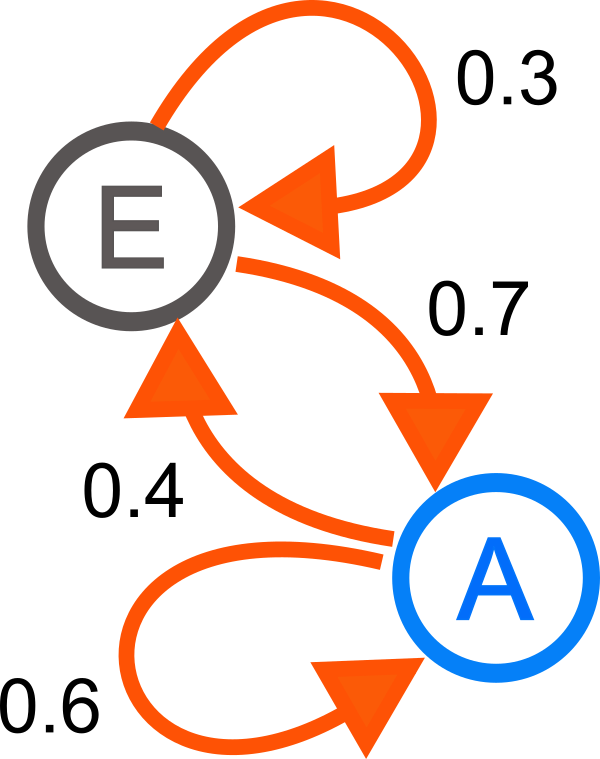
\includegraphics[scale=0.5]{markovketens.png}
  \label{fig:markovketens}
  \caption{Een simpele Markovketen\cite{markovketen}}
\end{figure}

Je kunt een Markovketen beschrijven als een gerichte graaf, waarbij de knopen de verschillende toestanden representeren en de pijlen de mogelijke overgangen representeren. De gewichten van de pijlen representeren de kans dat het systeem zich over die pijl 'beweegt' naar de volgende toestand. In Fig.~\ref{fig:markovketens} zien we een simpele Markovketen. Er zijn twee toestanden, E en A, en bij elke toestand twee pijlen: een pijl met een kans dat het systeem naar de andere toestand gaat en een pijl met een kans dat het systeem in dezelfde toestand blijft.

\subsection{Markovketens voor namen}

Je kunt het genereren van tekst of gewoon een naam ook beschrijven als een Markovketen, elke toestand is dan een letter en dan krijg je uit de volgorde van deze toestanden een naam. Verder heb je natuurlijk nog een eind en begin toestand nodig, want anders weet je niet wanneer je moet stoppen en bij welke staat je moet beginnen, deze toestanden noemen we EIND en BEGIN respectievelijk.

Laten we beginnen met een simpel voorbeeld waarin we alleen de letters 'e' en 'n' gebruiken, zie Fig.~\ref{fig:markovketens2}. Dit is al iets ingewikkelder dan Fig.~\ref{fig:markovketens}, maar het principe blijft hetzelfde.

Laten we beginnen bij BEGIN, vanuit daar zijn er twee mogelijkheden, we kunnen naar de 'e' of de 'n'. De kans dat we naar 'e' gaan is 0.6 en de kans voor 'n' 0.4. Dit hebben we zo gekozen, omdat we denken dat namen vaker met een 'e' beginnen dan met 'n'. Dezelfde soort keuzes hebben we moeten maken voor de pijlen vanuit 'e'. Er is een kleine kans dat dit het einde van het woord is en een grotere kans dat we nog een keer 'e' krijgen en een nog grotere kans dat we nu 'n' krijgen.

Al dit soort keuzes goed maken wordt al snel erg lastig, maar gelukkig zijn er manieren om een Markovketen als het ware te trainen met voorbeeldnamen, daarover komt later meer. Eerst gaan we nu bekijken hoe we met een dergelijke Markovketen een naam genereren.

\begin{wrapfigure}{r}{0.4\textwidth}
  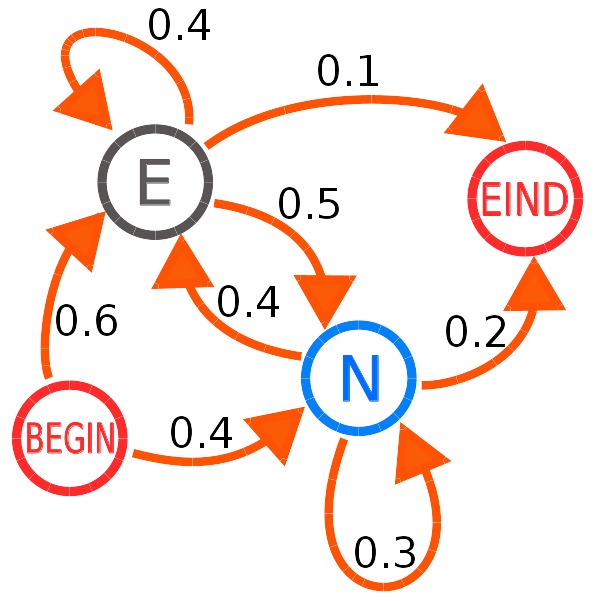
\includegraphics[width=0.9\linewidth]{markovketens2.png} 
  \caption{Een iets ingewikkeldere Markovketen, gebaseerd op Fig.~\ref{fig:markovketens}\cite{markovketen2}}
  \label{fig:markovketens2}
\end{wrapfigure}

We beginnen bij BEGIN, dan besluiten we willekeurig op basis van de kansen van de pijlen of we naar 'e' of 'n' gaan, laten we aannemen dat we deze keer naar 'n' gaan. Tot nu toe hebben we de naam “n”, vanaf hier kunnen we naar 'e', 'n' of EIND, we kiezen gebaseerd op de kansen willekeurig voor de 'e'. Nu hebben we de naam “ne”, nu kiezen we willekeurig uit 'e', 'n' en EIND met als uitkomst 'n'. Nu hebben we de naam “nen”, nu kiezen we wederom en krijgen we 'n'. We hebben nu de naam “nenn”, we kiezen nog een keer en krijgen EIND. Nu zijn we klaar en hebben we de naam “nenn” gegenereerd. Dit is natuurlijk niet een erg mooie naam en dat is grotendeels te wijten aan het feit dat we alleen de letters 'e' en 'n' gebruikten. Maar ook aan het feit dat de kansen die ik aan de pijlen heb gegeven niet optimaal zijn en natuurlijk ook aan ongeluk.

Als we dit proces nog een paar keer herhalen krijgen we elke keer een andere naam, dit proces doen we natuurlijk niet handmatig, want dat zou erg foutgevoelig en tijdrovend zijn, we hebben hiervoor een programmaatje geschreven, wat bijgevoegd is als simple-markov.scm. Een paar uitkomsten van dit programma zijn: “eeeeenn”, “ee”, “enenn”, “neneen”, “enen”, “eeenenenenennn”, “eene”, “enn”, “n” en “neeneneenen”.

\subsection{Markovketens trainen}

Het is lastig om handmatig de data voor een grotere Markovketen te bedenken. Niet alleen is het lastig om de bedenken wat de kans is om van de éne letter naar de ander te gaan, ook moet je dit heel vaak doen. Daarom is het handig om een Markovketen als het ware te trainen op voorbeeld namen. Hierbij haal je uit een zo groot mogelijke set van voorbeeld data de kansen waarmee elke letter elke andere letter opvolgt.

Voor dit doel hebben we een lijst van eiland namen samengesteld vanaf Wikipedia, die we daarna met behulp van wat programma's en ook gedeeltelijk handmatig schoon hebben gemaakt (dus bijvoorbeeld de coördinaten die er op Wikipedia achter stonden). Deze lijst is bijgevoegd als \texttt{names.txt}. Een aantal voorbeeld namen uit deze lijst zijn: “Loreto”, Porvenir”, “Tigre”, “Yaguas”, “Muñoz”, “Pernambuco”, “Margarita”, “Tigrera”, “Venezuela”, “Aduché”.


Als we hiermee een naïeve implementatie van een Markovketen voor namen mee trainen, krijgen we namen zoals: “Etibelangocharst”, “Lamarnd”, “Wochiouastr”, “Manngulledug”, “Murtascckbutégrockore”, “Webbbbamp Isayrna”, “Trocas”. Sommigen van deze namen, zoals “Trocas”, zijn redelijk goed, maar de meesten zijn zeer ongeloofwaardig. Zo heeft “Webbbbamp Isayrna” 4 b's achter elkaar. We zouden dit soort problemen kunnen verminderen door de namen te gaan controleren aan de hand van bepaalde criteria, zoals “niet meer dan twee keer dezelfde letter”, maar het is veel werk om alle mogelijke restricties zelf te bedenken. We willen liever dat de Markovketens zelf beter van de voorbeeldnamen leren zodat we betere namen krijgen.

Omdat de naïeve implementatie maar 1 letter 'onthoud' is er de mogelijkheid om meerdere keren dezelfde letter achter elkaar te krijgen of andere onmogelijke combinaties zoals “scckb” in “Murtascckbutégrockore”, terwijl deze in het voorbeeld niet eens voorkomen. Om dit te verhelpen kan je elke toestand niet laten afhangen van de laatste letter, maar van de laatste N letters. Bijvoorbeeld als je tot nu toe “Sch” hebt en N is 2, dan is de huidige toestand “ch” en kijk je niet naar alle de frequenties waarmee de letters alleen na de 'h' komen, maar naar de frequenties waarmee letters na de combinatie “ch” komen. Vervolgens kies je op basis daarvan de volgende letter, bijvoorbeeld de 'o'. Nu is de huidige toestand “ho” en kies je op basis daarvan een volgende letter, en zo ga je verder.

Hoe hoger N, hoe meer de gegenereerde namen op de voorbeeldnamen beginnen te lijken. Met een N van 5 en als trainingslijst \texttt{names.txt} (dat 1886 namen bevat) is zijn vrijwel alle namen in de output precies overgenomen uit de trainingslijst. Als we dat hadden gewild hadden we gewoon direct willekeurig uit de lijst kunnen kiezen! Dit probleem ontstaat omdat met een N van 5 de combinaties zoals “Tiriz” meestal maar één keer voorkomt in de trainingslijst, waardoor er maar één mogelijke volgende letter is, namelijk de 'i'. Dan heb je de toestand “irizi”, waarna alleen de 's' kan komen en met de toestand “rizis” die dan ontstaat kun je alleen de naam eindigen. Zo ontstaan telkens namen die precies in de trainingslijst voorkomen.

We willen dus een N kiezen waarmee de namen er zo echt mogelijk uit zien, maar zo min mogelijk precies hetzelfde zijn als voorbeeldnamen. Voordat we kiezen welke N hiervoor het beste is, bespreken we eerst onze implementatie van dit principe in C++.

\subsection{Implementatie}

Om dit algoritme in C++ te kunnen implementeren moeten we eerst bepalen hoe we de gegenereerde graaf zullen voorstellen. Hiervoor beginnen we bij de kleinste bouwsteen, een enkele knoop. Deze wordt opgeslagen in een struct met de naam \texttt{MarkovElement} die een aantal gegevens over de knoop opslaat, namelijk het totale aantal keer dat dit element voorgekomen is en een \texttt{map} waarin de pijlen vanuit de knoop opgeslagen worden.

Dit totaal aantal keren dat het element is voorgekomen is eigenlijk overbodig om op te slaan, in de map met pijlen wordt immers ook het aantal keer dat elk ander element na dit element voorkomt. Als je die allemaal optelt krijg je hetzelfde getal! De enige reden dat we dit aantal apart opslaan is om de computer wat tijd te besparen, die anders zou moeten worden besteed aan het langslopen van alle pijlen om ze bij elkaar op te tellen. Dit totaal aantal keren is namelijk nodig elke keer als de computer wil besluiten naar welke knoop na deze te gaan, hoe dat wordt gedaan bespreken we later.

Een \texttt{map} is een structuur die bepaalde \emph{keys} met bijbehorende \texttt{values} verbindt. Hierbij is het dus makkelijk om efficient de waarde die bij een bepaalde \emph{key} hoort op te vragen of te veranderen. De pijlen vanuit een \texttt{MarkovElement} worden opgeslagen in de vorm van een \texttt{map} met als keys de verschillende letters die op het element kunnen volgen en als \emph{value} het aantal keer dat de overgang naar die letter is voorgekomen.

De \texttt{map} voor het \texttt{MarkovElement} van de letter 'E' in het eerdere voorbeld (Fig.~\ref{fig:markovketens2}) zou bijvoorbeeld de volgende waarden kunnen bevatten:

\begin{lstlisting}
'E'  => 4
'N'  => 5
'\n' => 1
\end{lstlisting}

Het '\texttt{\textbackslash n}' hierin staat in computers voor het breken van een regel, een 'enter' dus. Omdat in namen nooit 'enters' voorkomen gebruiken we in onze implementatie de '\texttt{\textbackslash n}' om het einde van een naam aan te duiden.

In dit voorbeeld wordt een \texttt{N} gebruikt van 1, wat betekent dat de letters die in de \texttt{map} staan direct overeenkomen met de waarden van de knopen waar ze naar verwijzen. Bij een hogere \texttt{N} moet om de waarde van het corresponderende element de letter aan het eind van de huidige waarde worden gezet en de eerste letter van de waarde worden weggehaald. Als je bijvoorbeeld bij \texttt{N=3} een element “baz” hebt en wil weten waar de 'i' in de \texttt{map} naar verwijst, moet je eerst de 'i' aan het eind van “baz” toevoegen. Dan krijg je “bazi” en daar haal je de eerste letter vanaf, wat voor “azi” zorgt, wat de waarde is van de knoop waarnaar de 'i' verwijst.

\subsection{De Markov map}

We moeten al deze elementen op een manier opslaan zodat we ze makkelijk kunnen vinden aan de hand van de waarde van de knoop waarbij ze horen. 
\\\\
\textbf{Dit totaal aantal keren is namelijk nodig elke keer als de computer wil besluiten naar welke knoop na deze te gaan, hoe dat wordt gedaan bespreken we later.}

\newpage

\section{Hoogtekaart}

\subsection{Introductie}

De eerste stap in het generen van onze wereld is een initiële hoogtekaart maken. Daarmee bedoelen wij een representatie die voor elke plek de hoogte aangeeft. De bedoeling is dat deze hoogtekaart later door andere modules kan worden aangepast, de rivier module zou bijvoorbeeld een pad kunnen weg eroderen.

\begin{wrapfigure}{r}{0.4\textwidth}
  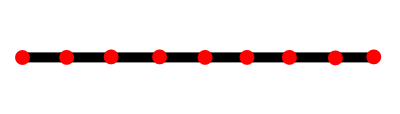
\includegraphics[width=0.9\linewidth]{hoogtekaart-line.png}
  \caption{\cite{hoogtekaart-illustratie}}
  \label{fig:hoogtekaart-line}
\end{wrapfigure}

Om de hoogtekaart te generen hebben we besloten een variant van het midpoint-displacement algoritme, het diamond-square algoritme te gebruiken. Dit algoritme is een verbeterde variant van het midpoint-displacement algoritme en genereert net als het midpoint-displacement algoritme een (semi-)fractal. De hoogtekaart die gegenereerd wordt heeft dus een vergelijkbare opbouw op elke schaal. Dit algoritme wordt daarom vaak gebruikt voor het genereren van een terrein aangezien een landschap op grote schaal (een berg) grofweg dezelfde vorm heeft als op kleine schaal (een rots).

Om het diamond-square algoritme voor een 2 dimensionale kaart uit te leggen is het handig om eerst het midpoint-displacement algoritme in 1 dimensie uit te leggen, aangezien het diamond-square algoritme een verbetering is van het midpoint-displacement algoritme voor 2 dimensies.

\subsection{Het midpoint-displacement algoritme in 1 dimensie}

\begin{wrapfigure}{r}{0.4\textwidth}
  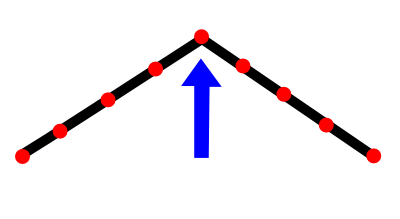
\includegraphics[width=0.9\linewidth]{hoogtekaart-midpoint.png}
  \caption{\cite{hoogtekaart-illustratie}}
  \label{fig:hoogtekaart-midpoint}
\end{wrapfigure}

Het midpoint-displacement algoritme werkt in 1 dimensie op een lijst van $2^n + 1$ punten, waarvan word aangenomen dat ze op een lijn allemaal even ver van elkaar af liggen, alle punten worden op een hoogte van 0 geplaatst. De startsituatie wordt in Fig.~\ref{fig:hoogtekaart-line} grafisch weergegeven. De 9 punten $(2^3 + 1)$ zijn in rood afgebeeld.

Vervolgens wordt het middelste punt met een willekeurige hoeveelheid (uniform verdeeld) naar omhoog of omlaag verplaatst. In Fig.~\ref{fig:hoogtekaart-midpoint} is te zien hoe het middelste punt naar boven is verplaatst. Alle punten die nog geen waarde hebben gekregen bewegen mee alsof een punt op een touw omhooggetrokken wordt.

\begin{figure}
  \centering
  \parbox{0.33\textwidth}{%
    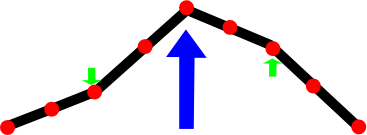
\includegraphics[width=0.9\linewidth]{hoogtekaart-mountain1.png}%
    \caption{\cite{hoogtekaart-illustratie}}%
    \label{fig:hoogtekaart-mountain1}}%
  \parbox{0.33\textwidth}{%
    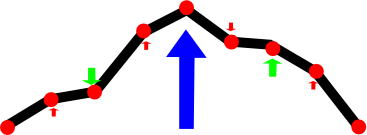
\includegraphics[width=0.9\linewidth]{hoogtekaart-mountain2.png}%
    \caption{\cite{hoogtekaart-illustratie}}%
    \label{fig:hoogtekaart-mountain2}}%
  \parbox{0.33\textwidth}{%
    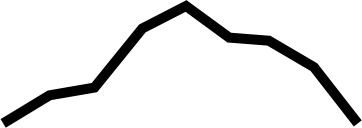
\includegraphics[width=0.9\linewidth]{hoogtekaart-mountain3.png}%
    \caption{\cite{hoogtekaart-illustratie}}%
    \label{fig:hoogtekaart-mountain3}}%
\end{figure}

De lijst wordt in deze fase in twee aparte lijsten opgedeeld, gesplitst op het middelste punt dat zojuist willekeurig bewogen is. Van beide van deze lijsten wordt weer het middelpunt genomen en willekeurig verplaatst (zie Fig.~\ref{fig:hoogtekaart-mountain1}). Nu is de verdeling van de afstand echter in een kleiner gebied, bijvoorbeeld tussen $-0.5$ en $0.5$ in plaats van $-1.0$ en $1.0$ bij het eerste middelpunt. Hoe kleiner de lijst wordt, hoe minder groot dit gebied ook zal zijn.. Hier wordt later meer over uitgelegd. Het is belangrijk om op te merken dat hoewel de hoogte in de figuren wordt aangegeven met een verplaatsing omhoog of omlaag, dit in het algoritme slechts een eigenschap van een punt is. Een punt zou dus ook niet loodrecht van de deellijst af verplaatsen maar nog steeds naar boven of beneden.

Ten slotte worden ook deze beide deellijsten weer opgedeeld en worden de laatste middelpunten willekeurig verplaatst (nog minder deze keer), zoals te zien is in Fig.~\ref{fig:hoogtekaart-mountain2}. Nu zijn er geen deellijsten meer te maken en is het algoritme klaar. Het eindresultaat is in Fig.~\ref{fig:hoogtekaart-mountain3} te zien.

\subsection{Het diamond-square algoritme}

\begin{wrapfigure}{r}{0.4\textwidth}
  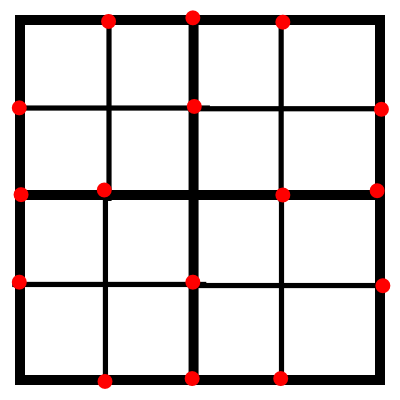
\includegraphics[width=0.9\linewidth]{hoogtekaart-2d.png}
  \caption{\cite{hoogtekaart-illustratie}}
  \label{fig:hoogtekaart-2d}
\end{wrapfigure}

Het standaard midpoint-displacement algoritme werkt goed in 1 dimensie, maar bij 2 of meer dimensies komt het sterk tekort. Omdat bij midpoint-displacement alleen het middelste punt met een willekeurige afstand wordt verplaatst, worden veel hoekpunten overgeslagen. In Fig.~\ref{fig:hoogtekaart-2d} zijn ter illustratie in rood de punten weergegeven die bij het standaard midpoint-displacement algoritme niet willekeurig worden verplaatst in dit 5 bij 5 grid. Ook wordt de positie van deze punten maar door 2 buurpunten bepaald, waar de middelpunten door 4 buren worden bepaald. Door deze eigenschappen van de punten heeft een 2 dimensionale versie van standaard middelpoint-displacement meer horizontale en verticale afwijkingen. Aangezien in de natuur geen voorkeur is voor een bepaalde richting zijn deze afwijkingen ook in onze hoogtekaarten ongewenst. 

Het diamond-square algoritme lost dit probleem op door een extra fase aan elke ronde toe te voegen. Na deze fase zijn de aangepaste punten gearrangeerd in een rooster van vierkanten, deze stap wordt daarom de square step genoemd. Bij de stap waar de middelpunten verplaatst worden zijn de aangepaste punten juist gearrangeerd in een rooster van 90 graden geroteerde vierkanten die diamanten worden genoemd. Deze stap heet dan ook de diamond step. Hiervan komt ook de naam van het diamond-square algoritme. In Fig.~\ref{fig:diamond-square}, afbeelding 1 tot 4, zijn de stappen van het diamond-square algoritme op een vijf bij vijf rooster weergegeven. In afbeelding 2 tot 4 zijn de diamond steps te zien; in adbeelding 3 tot 5 de square steps.

\begin{figure}[h!]
  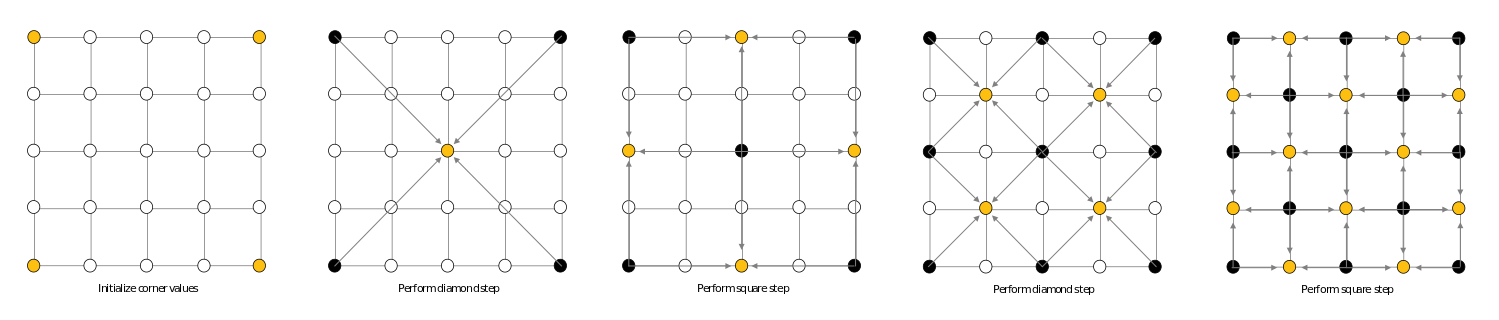
\includegraphics[width=\linewidth]{diamond-square.png}
  \caption{Visualisatie van de Diamond Square Algorithm\cite{diamond-square}}
  \label{fig:diamond-square}
\end{figure}

Alle punten op het behandelde rooster van het diamond-square algoritme worden 1 keer verplaatst. Het verplaatsen van punten in zowel de \emph{square step} als in de \emph{diamond step} is $O(1)$. Het totale algoritme is dus $O(1 * aantal~punten) = O(aantal~punten)$. Een algoritme met een een betere complexiteit om een hoogtekaart is niet mogelijk, aangezien elk punt voor een hoogtekaart een waarde toegewezen moet krijgen. Elk algoritme voor het genereren van een hoogtekaart is dus minimaal $O(aantal~punten)$. Deze goede complexiteit van het diamond-square algoritme is een belangrijk voordeel tegenover bijvoorbeeld fractal kaarten geproduceerd met verschillende lagen van \emph{perlin noise}, dat een complexiteit van $O(aantal~punten * log(aantal~punten))$ heeft.

\subsection{Relatie tussen verplaatsing en verplaatst gebied}

Zoals eerder al was genoemd, wordt het bereik van de willekeurige verplaatsing bij deze algoritmes vaak gerelateerd aan hoe groot het verplaatste gebied is. Over het algemeen wordt gekozen om een groter bereik te nemen bij een grotere functie. Aangezien de grootte van het verplaatst gebied van de ene stap naar de andere stap altijd halveert en de absolute grootte van de waardes niet uitmaakt (de kaart wordt immers genormaliseert), kan de hoeveelste stap het is worden gebruikt als een vervanger van de grootte van het verplaatst gebied. 

Vaak wordt het bereik van de verplaatsing vermenigvuldigt met $2^{-h*stap}$. De $h$ is hier een gekozen waarde, meestal tussen de $0.0$ en $1.0$. De $h$ kan worden veranderd om een ruigere kaart te genereren. Een lagere $h$ zorgt voor een ruigere kaart, het bereik wordt immers minder verkleint bij een kleiner verplaatst gebied, waardoor veel kleine details ontstaan. Een hogere $h$ zorgt voor een 'gladdere' kaart, waarbij er weinig kleine details zijn. Met een functie $r()$ die een willekeurig getal tussen $-1.0$ en $1.0$ geeft, is de verplaatsing van een punt met deze methode als volgt weer te geven:

\begin{equation}
  veerplaatsing~punt=r()*2^{-h*stap}
\end{equation}

Bij het gebruiken van deze simpele formule om het bereik van de willekeurige verplaatsing te bepalen liepen we echter tegen een probleem aan. De grote van de verandering van de verplaatsing bleek niet altijd direct gerelateerd aan de grootte van de verandering van het verplaatste oppervlakte. Op een schaal van honderden kilometers is namelijk geen grotere willekeurige verplaatsing dan op de schaal van bergen. En op een kleine schaal – bijvoorbeeld meters – is juist wel een kleinere verplaatsing dan op de schaal van bergen. Omdat de eerder gegeven formule altijd de willekeurige verandering vermenigvuldigt met een constante ($2^{-h}$), is deze formule niet geschikt.

\begin{figure}
  \centering
  \parbox[t]{0.33\textwidth}{%
    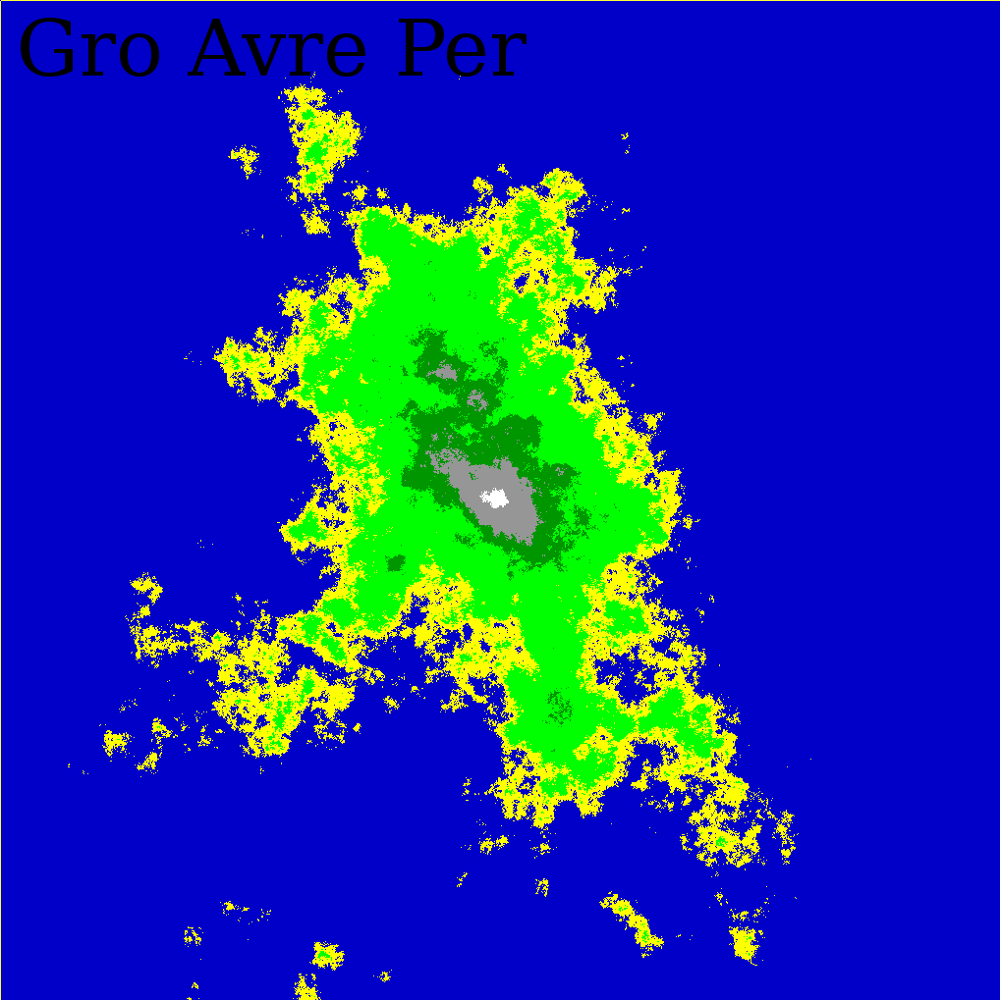
\includegraphics[width=0.9\linewidth]{kaart1.png}%
    \caption{$h=0.45$\cite{kaart}}%
    \label{fig:kaart1}}%
  \parbox[t]{0.33\textwidth}{%
    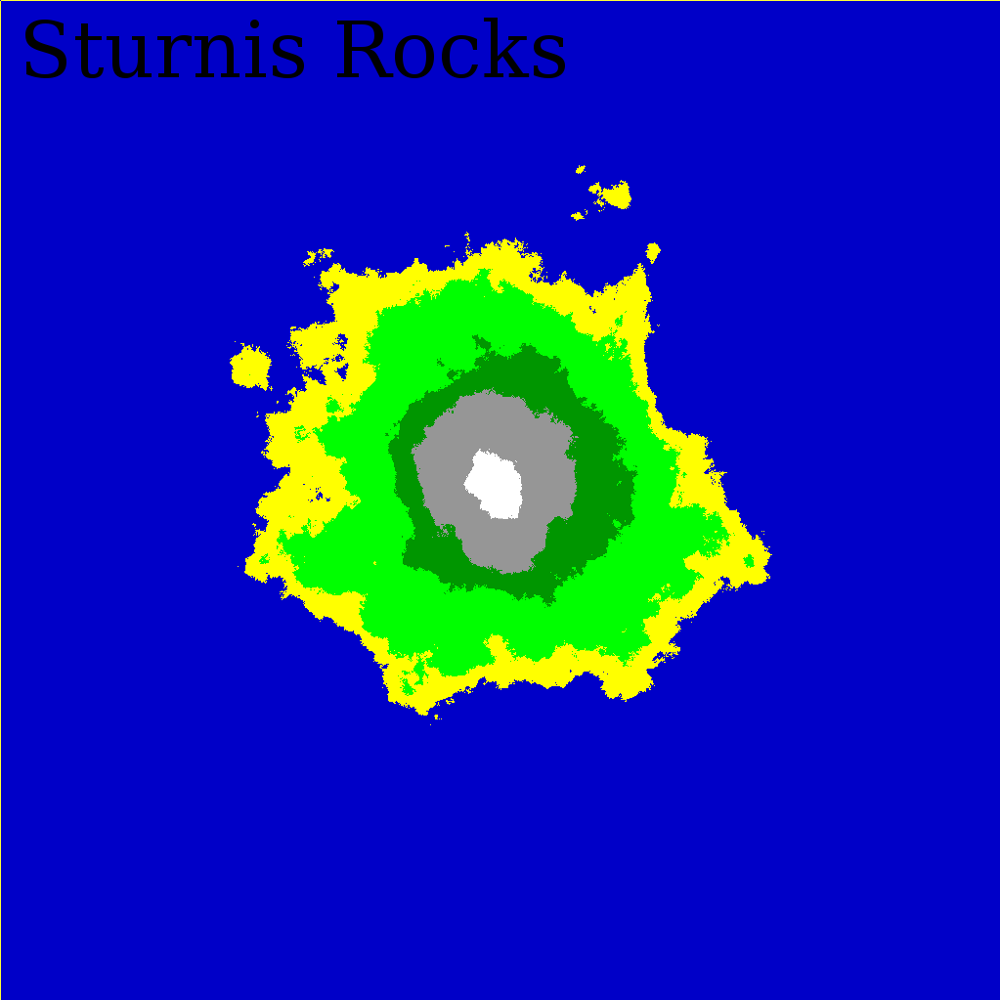
\includegraphics[width=0.9\linewidth]{kaart2.png}%
    \caption{$h=0.7$\cite{kaart}}%
    \label{fig:kaart2}}%
  \parbox[t]{0.33\textwidth}{%
    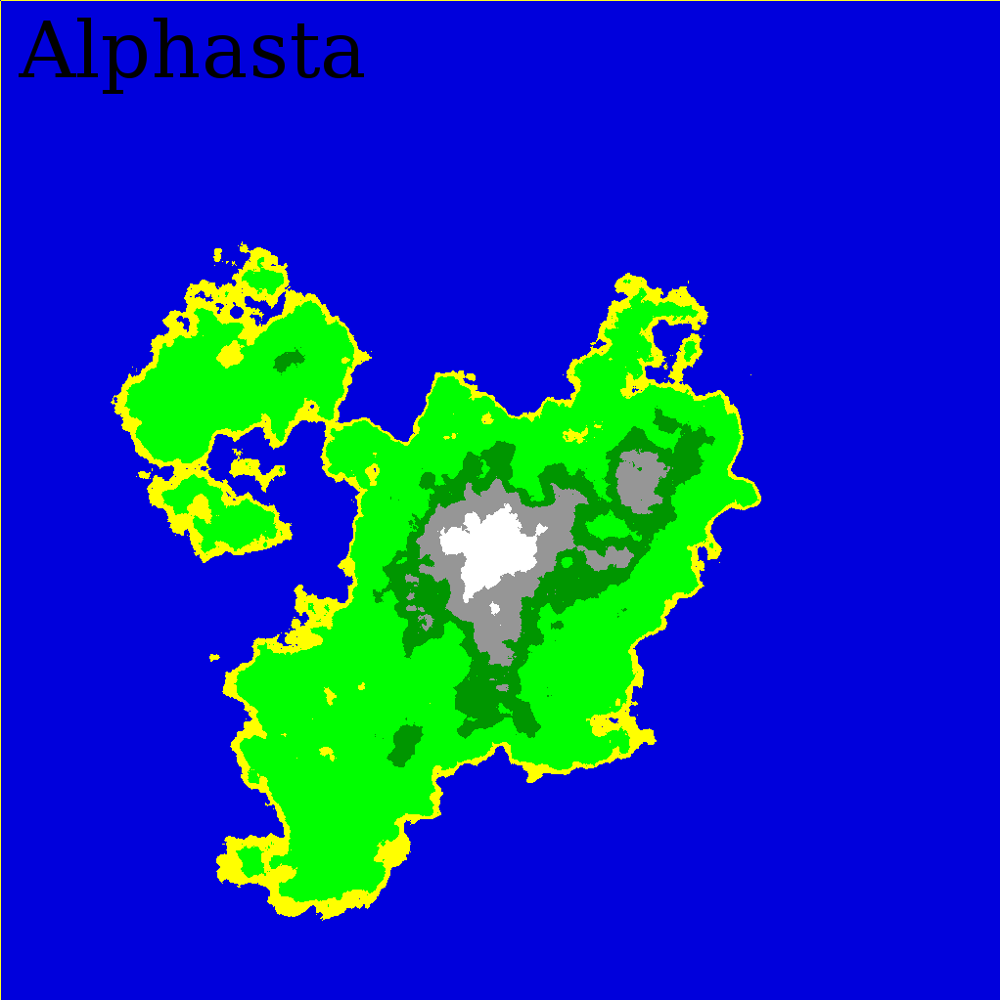
\includegraphics[width=0.9\linewidth]{kaart3.png}%
    \caption{\emph{aangepaste curve}\cite{kaart}}%
  \label{fig:kaart3}}%
\end{figure}

Dit probleem kwam ook naar voren in de kaarten die onze \emph{diamond-square} implementatie met deze formule genereerde. Bij een lage $h$ (een ruwe kaart), onstaan interessant gevormde eilanden, maar is er te sterk detail, wat voor te korrelige kusten zorgt (zie Fig.~\ref{fig:kaart1}). Bij een hoge h ontstaan wel zachte kusten, maar heeft het eiland bijna altijd dezelfde ronde vorm (zie Fig.~\ref{fig:kaart2}). Door de h te varieren was dit probleem niet op te lossen, dus zagen we ons genoodzaakt om een andere oplossing te bedenken. Wij hebben besloten een aangepaste curve te gebruiken waar we zelf kunnen bepalen wat het bereik is bij elke mogelijke grootte van het verplaatst gebied. Dit geeft ons volledige controle over de details en maakt het makkelijk om het later aan te passen. Helaas betekent dit wel dat we voor elke grootte van het verplaatst gebied moeten specificeren wat het bereik is, wat meer werk is dan een variabele aanpassen.

\subsection{Implementatie}

Ter illustratie hebben we een simpele implementatie van het diamond-square algoritme in C++11 geschreven. Dit programma schrijft een hoogtekaart naar een zwart-wit PNG-illustratie bestand dat met een gewone foto viewer bekeken kan worden. Dit programma gebruikt de lodepng library om naar PNG-bestanden te schrijven en is te vinden op: \url{http://paste.hydra.ws/p/o6R}.

\newpage
\bibliography{sources}

\end{document}
